\chapter{Tests}
\label{chap:Tests}

\subsection{UPPAAL schedulability analysis}
\label{sec:UPPAAL schedulability}
As described in Appendix \ref{sec:i3UPPAAL model}, Dumpsty contains three tasks: PrA, PrB and PrC. These three tasks all have individual WCET, which is not calculated, but rather tested, since calculating these through assembly proved to be impossible due to unbound loops in libraries. After testing the individual task's WCET, the worst case found would be significantly faster than what is labelled in UPPAAL, since the probability of hitting the actual worst case is close to impossible with the amount of tests done. In the following bulletpoints, all three tasks tested WCET and the WCET used in UPPAAL for the specific task is expressed, which is the first step to verify the schedulability of Dumpsty's tasks.

\begin{itemize}
	\item PrA \tab Tested: 1067 microseconds \tab UPPAAL: 2 milliseconds
	\item PrB \tab Tested: 732  microseconds \tab UPPAAL: 1 milliseconds
	\item PrC \tab	Tested: 8469 microseconds \tab UPPAAL: 9 milliseconds
\end{itemize}

For convenience, and to simplify the analysis, all tasks contain the worst case runtime of all interrupts and interrupt handlers that might occur during the execution of the task. These interrupts are generated by the motor encoders when Dumpsty is moving.

Figure \ref{UPPAAL Automata} depicts the automatas created in UPPAAL from two declared classes. The first class, task PrA, is the cyclic executive instance for the task PrA. The second class is simply a CPU which is the key needed to run the task. Every task can grab the CPU, but only one may hold it at any given time. The CPU is then released when the task is done executing, and another task can then proceed to run.

\begin{figure}[h]
	\centering
	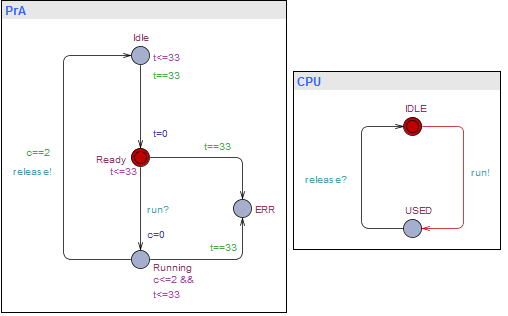
\includegraphics[scale=1]{billeder/UPPAALPr}
	\caption{Automata in UPPAAL}
	\label{UPPAAL Automata}
\end{figure}

In UPPAAL these automatas might have more than one instance, defined by the amount of tasks declared. In this case, there are three instances of the first class:

\begin{itemize}
	\item PrA = TASK(1, 33, 2);
	\item PrB = TASK(2, 33, 1);
	\item PrC = TASK(3, 33, 9);
\end{itemize}

The integers declared for every task have different meanings. These integers will be explained by the case task PrA. In task PrA, the integer 1 is the ID for the task, 33 is the deadline for the task in milliseconds, and 2 is the worst-case execution time for the task. The deadline for all tasks is the same, since this is the minimal interarrival-time(MIT) for coordinates from the Kinect sensor. All code has to be executed within the MIT of these coordinates, since a new coordinate will alter the path the robot choose.

The last step in the UPPAAL schedulability analysis is to use the verifier. This is done with two queries, found in listing \ref{Queries}. The first query checks if after some amount of time, greater than zero, all tasks has been executed at least once and all tasks are in the ready state. The second query checks that no task ever hits an error-state. If these two queries both succeed, the tasks can all be executed within the deadline, and the schedulability analysis is successful, and in this case, with tasks PrA, PrB and PrC, the tasks are schedulable within the deadlines.

\begin{lstlisting}[caption={Queries for UPPAAL}, label={Queries}]
E<> PrA.Ready and PrB.Ready and PrC.Ready and PrA.t==0 and PrB.t==0 and PrC.t==0 and time>0
E[] not (PrA.ERR or PrB.ERR or PrC.ERR)
\end{lstlisting}
